\documentclass[11pt, spanish]{report}
\usepackage[spanish]{babel}
\usepackage[utf8]{inputenc}
\usepackage{geometry}
\usepackage{graphicx}
\usepackage{subfig}
\usepackage{caption}
\usepackage{subcaption}
 \geometry{
 a4paper,
 total={170mm,257mm},
 left=20mm,
 top=20mm,
 }
\usepackage{graphicx}
\graphicspath{ {images/} }
\usepackage[utf8]{inputenc}
\decimalpoint

\title{Actividad8}
\author{César Andrés Pérez Robinson }
\date{Mayo 2019}

\begin{document}

\maketitle

\section{Introducción}
En esta actividad se pide trabajar con dos conjuntos de datos: los datos meteorológicos de la estación de Nogal con los que se trabajó en la actividad anterior, y otro conjunto de datos del suelo de la misma estación. Estos últimos son variables medidas con sensores bajo el suelo. \\ Las variables con las que estaremos trabajando son las temperaturas del suelo a 10, 20, 40 y 85 centímetros.
\section{Código desarrollado}
Primero se suben los archivos de datos a Jupyter Notebook, para el archivo de datos meteorológicos, al igual que en la actividad siete, se eliminan aquellas columnas 'Unnamed' y se agregan las columnas de 'MES', 'DIA', 'HORA' y 'MINUTO'. Se aprovechan los datos de cada 30 minutos utilizando:
\begin{verbatim}
dfm = dfm[((dfm['MINUTO'] == 30.0) | (dfm['MINUTO'] == 0.0) ) & 
         (dfm['FECHA']<'2010-01-01 00:30:00')]
dfm = dfm.reset_index(drop=True)
\end{verbatim}
Del segundo archivo de datos, se eliminan las columnas que no son de interés. Ya que queremos agregar también una columna de fecha al segundo DataFrame, donde las mediciones sean cada 30 minutos, se hace uso de un de un arreglo donde se obvserva la variable '4 Hour\_Minute\_RTM  L', la que puede ser de cuatro, tres o dos dígitos, donde los últimios dos dígitos van de 00 a 30, y significa que han pasado 30 minutos. Por lo tanto el primer o los primeros dos dígitos indican las horas. Por ejemplo, obtener el dato '230' significa que son las 2:30 am, y '1500' indica que son las 15:00 (3:00 pm). \\
Por lo tanto se usan if, else y elif para primero determinar si contiene dos, tres o cuatro dígitos la variable, una vez que se hace eso se utiliza append para asignar valores a las horas y minutos. Esto se usa con lo siguiente;
\begin{verbatim}
horas = []
minutos = []

for i in range(0,len(dfs)):
    if (len(str(dfs['4 Hour_Minute_RTM  L'][i]))==4):
        if (str(dfs['4 Hour_Minute_RTM  L'][i])[0:2]=='24'):
            horas.append('0')
            minutos.append('0')
            # De esta manera, al encontrar 4 dígitos en el valor de 
            # la columna, ubicamos aquellos que inicien con 24 como
            # el lugar donde se vuelve a inicar el conteo, por eso 
            # se utiliza append con el valor dado '0'
        else:
            h = str(dfs['4 Hour_Minute_RTM  L'][i][0:2])
            m = str(dfs['4 Hour_Minute_RTM  L'][i][2:4])
            horas.append(h)
            minutos.append(m)
            # por el contrario, cuando no inician con 24, tomamos el dato
            # de los primeros dos dígitos (horas) y los agregamos al str horas
            # y los ultimos dos dígitos (minutos) se agregan al str minutos
    elif(len(str(dfs['4 Hour_Minute_RTM  L'][i]))==3):
            h = str(dfs['4 Hour_Minute_RTM  L'][i][0:1])
            m = str(dfs['4 Hour_Minute_RTM  L'][i][1:3])
            horas.append(h)
            minutos.append(m)
    
            # En este caso, si se encuentran 3 dígitos en la columna, lo que se
            # tiene que hacer es tomar el valor del primer dígito como la hora
            # y los últimos dos como los minutos
    elif(len(str(dfs['4 Hour_Minute_RTM  L'][i]))==2):
            h = '0'
            m = str(dfs['4 Hour_Minute_RTM  L'][i][0:2])
            horas.append(h)
            minutos.append(m)
            # por último, si la columna tiene dos dígitos, el valor de hora
            # se encuentra fijo en '0' mientras que el de minutos toma los 
            # ultimos dos.
            
# Mientras tanto, los dias se mantienen estables
dias =[dfs['3 Day_RTM  L'][i] for i in range(0,len(dfs))]
\end{verbatim}
Se hace que cada vez que pasen 24 horas se tome como un día agregado. Se organiza de tal manera que se pueda agregar la variable de FECHA a ambos archivos de datos y después unirlos con la misma, usando;
\begin{verbatim}
# Se unen ambos dfm y dfs a partir de la variable FECHA
dfu = pd.merge(dfm, dfs, on=['FECHA'])
\end{verbatim}
Después nos quedamos con las columnas que son de nuestro interés;
\begin{verbatim}
    dfu = dfu.filter(['FECHA','Tsuelo_10cm','Tsuelo_20cm','Tsuelo_30cm',
                  'Tsuelo_40cm','Tsuelo_55cm','Tsuelo_70cm',
                  'Tsuelo_85cm','Tsuelo_100cm','t_Avg','air_Avg',
                  'net_rad_Avg','airT_Avg'],axis=1)
\end{verbatim}
Después se selecciona solamente el día 15 de Enero para crear las gráficas.
\begin{verbatim}
# Hago un dataframe del día que me interesa (15)
Dia15 = dfu['2009-01-15 00:00:00'<=dfu['FECHA']]
Dia15 = Dia15['2009-01-16 00:00:00'>dfu['FECHA']]
#Selecciono solamente las columnas de interés
Dia15i = Dia15.filter(['Tsuelo_10cm','Tsuelo_20cm',
                      'Tsuelo_40cm','Tsuelo_85cm',],axis=1)
\end{verbatim}
Para la Figura 1 se muestran las temperaturas del subsuelo el día 15 de Enero 2019.
\begin{figure}[ht]
\caption{Temperaturas a distintas profundidades}
\centering
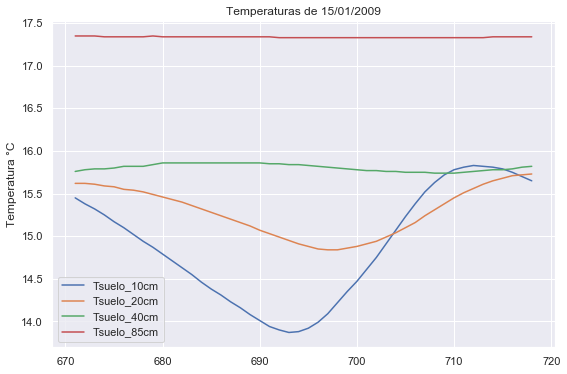
\includegraphics[width=0.65\textwidth]{figura1.png}
\end{figure}
Mientras tanto, para la temperatura del aire del día 15 se muestra la Figura 2.
\begin{figure}[ht]
\caption{Temperatura del aire}
\centering
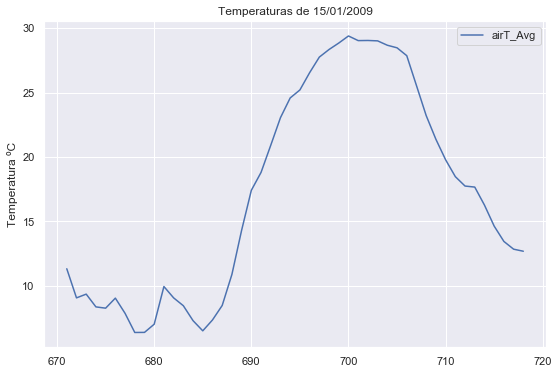
\includegraphics[width=0.65\textwidth]{figura2.png}
\end{figure}
Para realizar la Figura 3, que muestra las máximas, mínimas y promedio de temperaturas del suelo a 10 cm se tuvo que crear un dataframe que contenga temperaturas máximas, mínimas y promedio, usando:
\begin{verbatim}
dfa=dfu

#Primero crearemos variables para día y mes
dfa['DIA']=dfa['FECHA'].dt.day
dfa['MES']=dfa['FECHA'].dt.month

# se necesita un dataframe que contenga las temperaturas maximas minimas y promedio de cada 
# temperatura del subsuelo, por lo tanto se crean nuevos dataframes

#Para Tsuelo_10cm 
df10=dfa.filter(['DIA','MES','Tsuelo_10cm'],axis=1)
#tmin, tmax y tprom
df10["Tsuelo_10cm_max"] = np.round(df10.groupby(["MES","DIA"])
["Tsuelo_10cm"].transform("max"),decimals=1)
df10["Tsuelo_10cm_min"] = np.round(df10.groupby(["MES","DIA"])
["Tsuelo_10cm"].transform("min"),decimals=1)
df10["Tsuelo_10cm_prom"] = np.round(df10.groupby(["MES","DIA"])["Tsuelo_10cm"].transform("mean"),decimals=1)

#Para Tsuelo_20cm  
df20=dfa.filter(['DIA','MES','Tsuelo_20cm'],axis=1)
#tmin, tmax y tprom
df20["Tsuelo_20cm_max"] = np.round(df20.groupby(["MES","DIA"])
["Tsuelo_20cm"].transform("max"),decimals=1)
df20["Tsuelo_20cm_min"] = np.round(df20.groupby(["MES","DIA"])
["Tsuelo_20cm"].transform("min"),decimals=1)
df20["Tsuelo_20cm_prom"] = np.round(df20.groupby(["MES","DIA"])["Tsuelo_20cm"].transform("mean"),decimals=1)

#Para Tsuelo_40cm 
df40=dfa.filter(['DIA','MES','Tsuelo_40cm'],axis=1)
#tmin, tmax y tprom
df40["Tsuelo_40cm_max"] = np.round(df40.groupby(["MES","DIA"])
["Tsuelo_40cm"].transform("max"),decimals=1)
df40["Tsuelo_40cm_min"] = np.round(df40.groupby(["MES","DIA"])
["Tsuelo_40cm"].transform("min"),decimals=1)
df40["Tsuelo_40cm_prom"] = np.round(df40.groupby(["MES","DIA"])["Tsuelo_40cm"].transform("mean"),decimals=1)

#Para Tsuelo_85cm 
df85=dfa.filter(['DIA','MES','Tsuelo_85cm'],axis=1)
#tmin, tmax y tprom
df85["Tsuelo_85cm_max"] = np.round(df85.groupby(["MES","DIA"])
["Tsuelo_85cm"].transform("max"),decimals=1)
df85["Tsuelo_85cm_min"] = np.round(df85.groupby(["MES","DIA"])
["Tsuelo_85cm"].transform("min"),decimals=1)
df85["Tsuelo_85cm_prom"] = np.round(df85.groupby(["MES","DIA"])["Tsuelo_85cm"].transform
    ("mean"),decimals=1)


# se elimina aquello que no se va a graficar
df10 = df10.drop(['Tsuelo_10cm','DIA','MES'], 1)
df40 = df40.drop(['Tsuelo_40cm','DIA','MES'], 1)
df20 = df20.drop(['Tsuelo_20cm','DIA','MES'], 1)
df85 = df85.drop(['Tsuelo_85cm','DIA','MES'], 1)
\end{verbatim}
El uso de los archivos de datos generados se presentan en la Figura 3, que indican la temperatura a 10 cm.
\begin{figure}[ht]
\caption{Temperatura a 10cm}
\centering
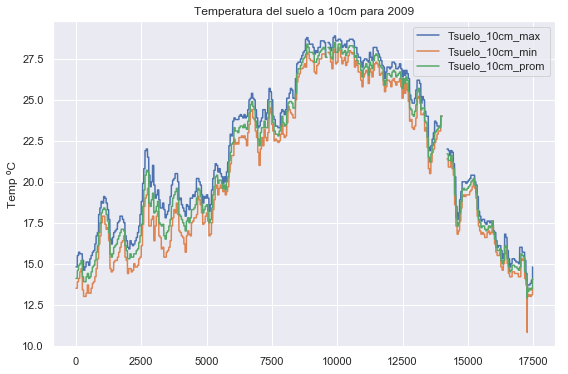
\includegraphics[width=0.65\textwidth]{figura3.png}
\end{figure}
Mismo que ocurre para la Figura 4, Figura 5 y Figura 6.
\begin{figure}[ht]
\caption{Temperatura a 20cm}
\centering
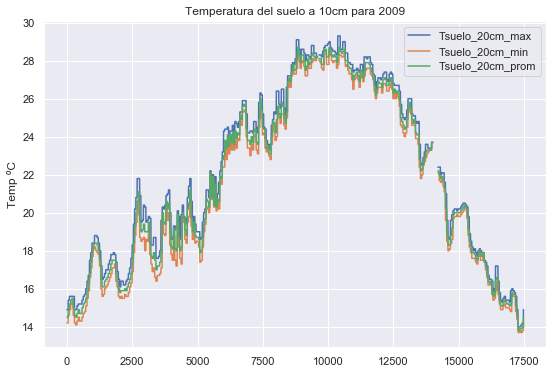
\includegraphics[width=0.65\textwidth]{figura4.png}
\end{figure}\begin{figure}[ht]
\caption{Temperatura a 40cm}
\centering
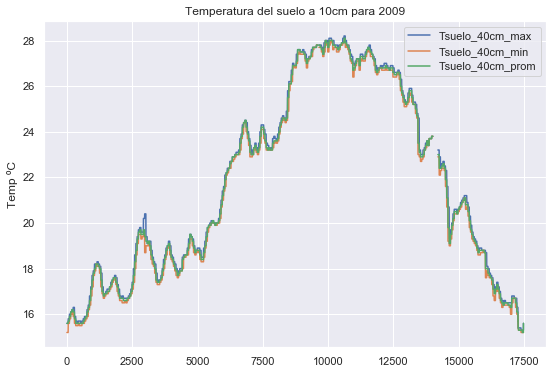
\includegraphics[width=0.65\textwidth]{figura5.png}
\end{figure}\begin{figure}[ht]
\caption{Temperatura a 85cm}
\centering
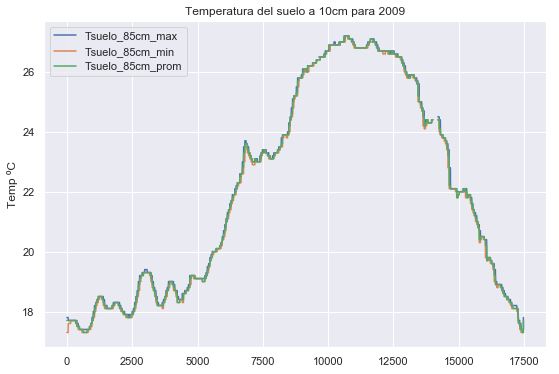
\includegraphics[width=0.65\textwidth]{figura6.png}
\end{figure}
\end{document}
